\section{Experimentacion y resultados}
En esta sección, se describen los experimentos realizados y los resultados
obtenidos en función del bentchmark. Se explicará el proceso de experimentación,
como se ha relizado y configurado el hypertuning, y los resultados obtenidos.\medskip

Además, los resultados obtenidos se analizaran de marnera crítica, 
comparándolos con la literatura existente y estableciendo conclusiones y 
posibles implicaciones para futuras investigaciones. En definitiva, el 
apartado de experimentación y resultados es una parte fundamental para 
demostrar la validez y la relevancia de la investigación realizada.

\subsection{Optimización de Hiperparámetros}
La optimización de hiperparámetros se refiere al proceso de ajustar los parámetros 
de entrenamiento y configuración de un modelo de Machine Learning con el objetivo de 
mejorar su desempeño. Los hiperparámetros son variables que no se aprenden automáticamente 
a partir de los datos, sino que deben ser configurados por el investigador.\medskip

En un modelo de Machine Learning, los hiperparámetros pueden incluir variables como 
la tasa de aprendizaje, la profundidad de la red neuronal, la cantidad de neuronas en 
cada capa, el tamaño del Batch, entre otros. El proceso de optimización implica la 
selección cuidadosa de los valores de los hiperparámetros que maximicen el rendimiento 
del modelo en un conjunto de datos de prueba. Esto generalmente se realiza mediante 
la búsqueda de un rango de valores posibles para los hiperparámetros y evaluando el 
rendimiento del modelo en cada combinación posible.\medskip

La optimización de hiperparámetros es un aspecto importante del desarrollo de modelos 
, ya que una mala selección de hiperparámetros puede llevar a un modelo con un rendimiento 
deficiente. Un modelo que esté bien optimizado puede mejorar significativamente su 
capacidad para hacer predicciones precisas y generalizar a datos nuevos y desconocidos.

\subsubsection{Optimización de Hiperparámetros con Optimización Bayesiana}
La optimización bayesiana es un método de optimización de hiperparámetros para modelos 
de Machine Learning que utiliza un enfoque probabilístico para buscar el conjunto 
óptimo de hiperparámetros. En lugar de evaluar todas las combinaciones posibles de 
hiperparámetros, la optimización bayesiana utiliza una estrategia de búsqueda más 
inteligente que utiliza la información de iteraciones anteriores para buscar en el 
espacio de búsqueda de manera más eficiente.\medskip

La optimización bayesiana comienza con una función subrogacion que mide la calidad del modelo 
en un conjunto de datos de prueba. La estrategia de optimización bayesiana consiste en construir 
un modelo probabilístico de la función objetivo y utilizarlo para decidir qué hiperparámetros 
probar a continuación. En cada iteración, el modelo actualizado sugiere un conjunto de 
hiperparámetros que se espera que tengan una buena probabilidad de mejorar el rendimiento 
del modelo. El modelo se entrena con los nuevos hiperparámetros y se evalúa 
su rendimiento en el conjunto de prueba. Esta evaluación se utiliza para actualizar el 
modelo probabilístico, y se repite el proceso de búsqueda de hiperparámetros hasta 
que se encuentra una combinación que satisfaga el criterio de parada.

\subsubsection{Aplicación de Optimización Bayesiana con Optuna}
Optuna utiliza el método de optimización bayesiana para buscar el conjunto óptimo de
hiperparámetros. Además, mediante Optuna-Dashboard se puede visualizar el proceso de
optimización, la importancia de cada hiperparámetro, la relación entre los hiperparámetros
y llevar un registro de las mejores combinaciones de hiperparámetros encontradas.\medskip

A continuación se muestra el listado de hiperparámetros:

\begin{table}[ht]
    \centering
    \begin{tabular}[ht]{l|c|c} 
        \textbf{Lista de Hiperparámetros} & \textbf{Rango de valores} & \textbf{Valor Optimo}\\
        \hline
        \textbf{Número de instancias pequeñas} & 0 -- 20k & 20k\\
        \textbf{Número de instancias medianas} & 0 -- 20k & 10k\\
        \textbf{Número de instancias grandes}  & 0 -- 20k & 10k \\
        \textbf{Tasa de aprendizaje} & 0.00001 -- 0.001 & 15 \\
        \textbf{Número de épocas} & 5 -- 35 & 30 \\ 
        \textbf{Número de episodios} & 1 -- 3 & 2 \\
        \textbf{Tamaño del Batch} & 64, 128, 256 & 64\\
        \textbf{Canales ocultos} & 100 -- 300 & 200 \\
        \textbf{Número de capas ocultas} & 1 -- 6 & 1 \\
    \end{tabular}
    \caption{Lista de hiperparámetros}
    \label{tab:hyperparams}
\end{table}

Esta lista de hiperparámetros se obtuvo a partir de múltiples experimentos. En cada 
experimento se realizaban tres entrenamientos con los mismos hiperparámetros y luego
se promediaba el resultado de cada métrica, para así obtener un resultado más estable.
El objetivo de estos experimentos era minimizar la función objetivo y se realizaron
un total de 300 pruebas con diferentes combinaciones. En la figura \ref{fig:experiments}
se puede observar la visualización de los experimentos realizados y como progresa la
configuración de los hiperparámetros, aquí los puntos azules representan los experimentos
realizados y la linea roja representa la mejor combinación de hiperparámetros encontrada
hasta el momento.

\begin{figure}[ht]
    \centering
    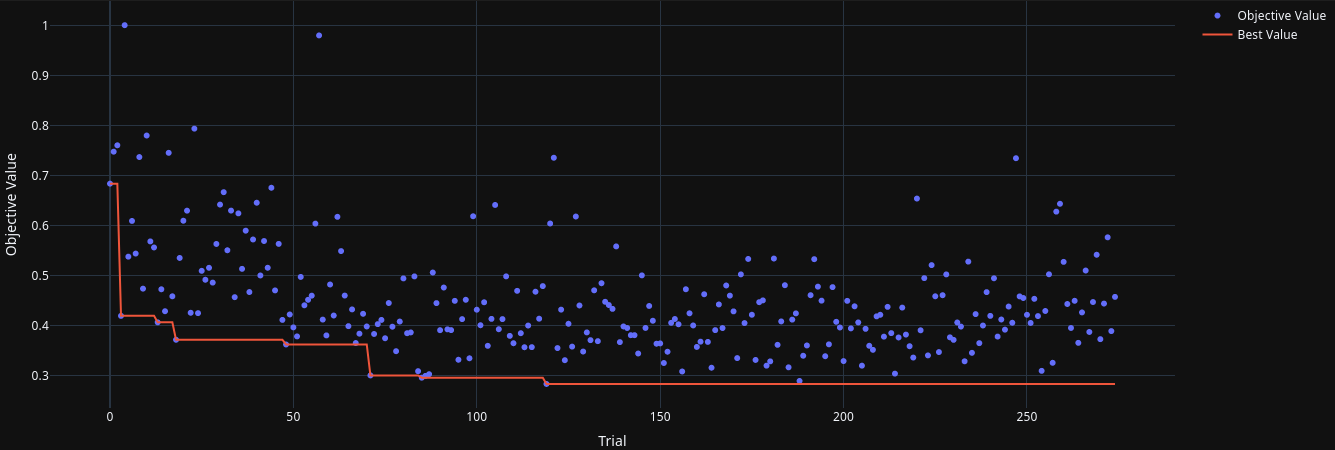
\includegraphics[scale=0.31]{experiments.png}
    \caption{Visualización de la experimentación de hiperparámetros}
    \label{fig:experiments}
\end{figure}

Una de las ventajas de utilizar Optuna es que se puede visualizar la importancia de cada
hiperparámetro, en la figura \ref{fig:importance} se puede observar que los hiperparámetros
que mayor impacto tienen en el rendimiento del modelo son la tasa de aprendizaje, el número
de instancias pequeñas y el número de capas ocultas. Este conocimiento ha traído consigo
una mejora en el rendimiento del modelo, en este caso debido a que se ha visto que el
número optimo de capas ocultas es 1, ha supuesto una mejora en la velocidad del modelo
ya que no solo se reduce el tiempo de entrenamiento sino que también se reduce el tiempo
de procedimiento a la hora de realizar predicciones.

\begin{figure}[ht!]
    \centering
    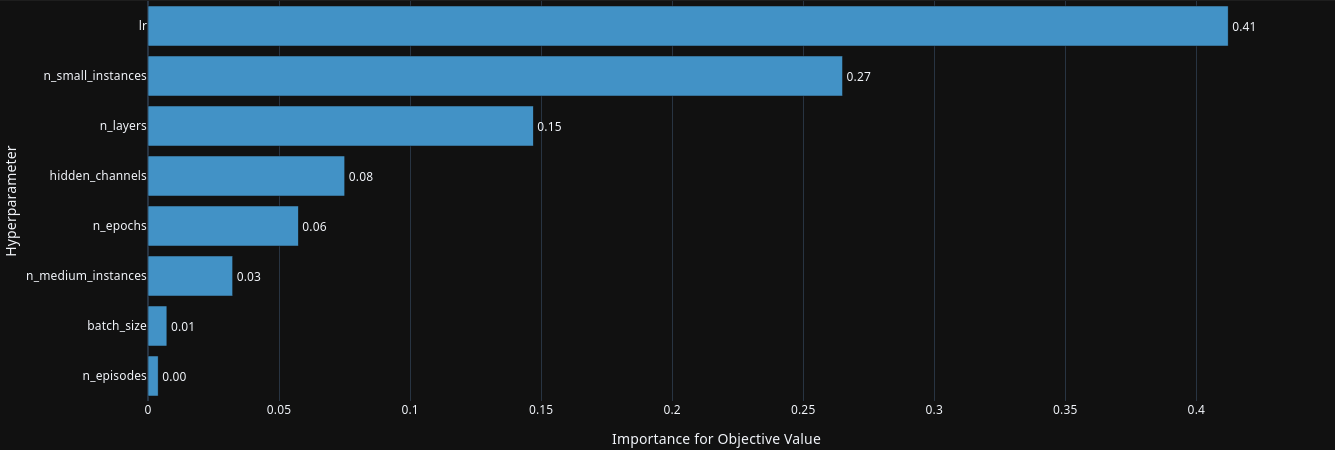
\includegraphics[scale=0.31]{importance.png}
    \caption{Importancia de los hiperparámetros}
    \label{fig:importance}
\end{figure}

\subsection{Análisis de los resultados}
En esta sección se analizarán los resultados obtenidos durante las diferentes
fases del proceso de desarrollo del proyecto. Se compararán los resultados
obtenidos con los resultados de la literatura existente, y se establecerán
conclusiones y posibles implicaciones para futuras investigaciones.

\begin{table}[ht]
    \centering
    \begin{tabular}[ht]{|l|cccc|}
        \hline
                  & Modelo v0 & Modelo v1 & Modelo v2 & Modelo v3 \\
        \hline
        MK01      & 2.850    & 0.923    & 0.225    & 0.075    \\
        MK02      & 3.661    & 0.191    & 0.423    & 0.346    \\
        MK03      & 3.583    & 0.850    & 0.240    & 0.073    \\
        MK04      & 1.877    & 0.494    & 0.450    & 0.283    \\
        MK05      & 8.578    & 1.122    & 0.104    & 0.133    \\
        MK06      & 8.578    & 1.122    & 0.754    & 0.747    \\
        MK07      & 3.143    & 1.288    & 0.287    & 0.273    \\
        MK08      & 2.809    & 0.246    & 0.130    & 0.032    \\
        MK09      & 5.302    & 0.567    & 0.156    & 0.198    \\
        MK10      & 6.898    & 0.786    & 0.704    & 0.535    \\
        \hline
        Calc time & 03:00    & 01:03    & 01:17    & 01:37    \\
        AVG       & 4.282    & 0.709    & 0.347    & 0.269    \\
        \hline
    \end{tabular}
    \caption{Tabla con los resultados del modelo}
\end{table}

En la siguiente tabla se muestran los resultados obtenidos por las
diferentes versiones del modelo, y el tiempo total de procesamiento
para completar todo el proceso de bentchmark. A continuación vamos a
explicar el desempeño de cada una de las versiones del modelo.
\begin{itemize}
    \item \textbf{Modelo v0:} Esta versión del modelo es la primera que se
        desarrolló, y la que se utilizó para realizar las pruebas de
        concepto. Como se puede observar, los resultados obtenidos son
        muy malos, y el tiempo de procesamiento es muy elevado. Esto
        se debe a que el modelo no está bien formulado, y es una base
        para el desarrollo e iteracion de las siguientes versiones.
    \item \textbf{Modelo v1:} Esta versión del modelo es la primera que
        se desarrolló con el objetivo de obtener resultados. Como se
        puede observar, los resultados obtenidos son muy buenos, y el
        tiempo de procesamiento es muy bajo. Esto se debe a que se han
        realizado mejoras internas en el modelo y se ha aplicado una
        normalizacion más sofisticada a los datos de entrada, lo que
        ha permitido obtener mejores resultados.
    \item \textbf{Modelo v2:} Para esta version hubo un cambio en el
        environment, se cambio el paradigma de prediccion y en vez
        de predecir a nivel de operaciones, se predice a nivel de
        la relación entre maquinas y operaciones. Esto ha permitido
        reducir la complejidad del espacio de decisiones y obtener
        mejores resultados.
    \item \textbf{Modelo v3:}
\end{itemize}


\begin{table}[ht]
    \centering
    \begin{tabular}[ht]{|l|cccc|}
        \hline
                  & spt & lwkr & mwkr & tabl \\
        \hline
        MK01      & 65      & 76    & 54    & 49    \\
        MK02      & 44      & 48    & 41    & 41    \\
        MK03      & 397     & 506   & 296   & 263   \\
        MK04      & 109     & 121   & 89    & 89    \\
        MK05      & 231     & 291   & 188   & 188   \\
        MK06      & 128     & 143   & 139   & 128   \\
        MK07      & 188     & 238   & 262   & 188   \\
        MK08      & 670     & 1042  & 558   & 523   \\
        MK09      & 573     & 723   & 536   & 444   \\
        MK10      & 536     & 627   & 524   & 363   \\
        \hline
    \end{tabular}
    \caption{Resultados de las reglas de ordenación}
\end{table}

\begin{itemize}
    \item \textbf{spt:} Shortest Processing Time
    \item \textbf{lwkr:} Longest Work Remaining
    \item \textbf{mwkr:} Most Work Remaining
    \item \textbf{tabl:} Tabu Search
\end{itemize}


\subsection{Otras representaciones del problema}
Durante el desarrollo de este trabajo se han probado diferentes representaciones
del problema con el objetivo de buscar la que mejor se adapte al caso particular del FJSP. En
esta sección se van a explicar las diferentes representaciones que se han probado
y se han terminado por descartar, junto con una breve explicación de las razones
por las que se han descartado y que características de ellas se han aprovechado
para la representación final. Por último, se explicará de forma breve como se
modeló su espacio de estados y de acciones, y como se actualizaba el estado
de forma breve para cada una de ellas. 

\subsubsection{Representación con construcción secuencial}
Esta representación es la primera que se probó, y consiste en representar el
problema de una forma secuencial, es decir, cada operación se asigna a una máquina
en función de la información que se tiene en ese momento. Esta idea 
sentó las bases de como se podría representar el proceso de construcción de una
solución, pero se descartó por ser demasiado simple y tener problemas de escalabilidad,
ya que no existía una forma de proveer adecuadamente toda la información necesaria
para la toma de decisiones. A continuación, se explicara su implicación.

\begin{itemize}
    \item \textbf{Espacio de estados:} el estado es representado por una 
    lista de máquinas, donde cada máquina tiene una lista de operaciones asignadas
    a ella. Se utiliza una estructura de datos matricial donde se proporcionan estadísticas 
    sobre la máquina que esta asignada para representar este estado. Ademas, cada elemento de la lista 
    contiene información sobre las operaciones, su duración, prioridad u otras características relevantes.
    \item \textbf{Espacio de acciones:} Las acciones posibles consisten en asignar una operación 
    a una máquina específica o realizar un cambio de máquina. Es posible representar las acciones 
    mediante un conjunto de códigos que identifiquen cada operación. En este caso, las acciones
    disponibles se mostrarían junto a un código extra que representaría el cambio de máquina, este código
    tomo al valor de la ultima operación más uno.
    \item \textbf{Transiciones de estado:} Cuando el agente asigna una operación a una máquina, 
    el estado se actualiza con la nueva asignación. Si el agente decide cambiar de máquina, 
    el estado se actualiza para reflejar la nueva máquina activa y las operaciones pertinentes.
\end{itemize}

\subsubsection{Representación mediante imagen con eliminación}
Esta representación consiste en representar el problema mediante una imagen, donde
cada píxel representa el tiempo de finalización de una operación en una posición
específica. El modelo en cuestión se basa en ir eliminando las operaciones de la
imagen que se encuentran ya asignadas en las diferentes máquinas en todas las
posiciones, el objetivo es eliminar todas las operaciones sobrantes de la 
imagen.\medskip

Esta representación se descartó por ser demasiado compleja, ya que aunque
en un principio parecía que podría ser una buena representación debido a la naturaleza
gráfica del problema, la complejidad de la representación y la gran dimensionalidad de
la misma la hacían inviable. No se rescató ninguna característica de esta para la 
representación final, ya que no se encontró ninguna que pudiera ser útil. Aquí se
explicará de forma breve como se modeló.

\begin{itemize}
    \item \textbf{Espacio de estados:} El estado se representa por una imagen que contiene 
    los posibles tiempos de finalización de las operaciones. Existe una matriz de píxeles 
    para representar la imagen, donde cada píxel representa el tiempo asociado a una operación 
    en una posición específica. Por ejemplo, el valor de un píxel podría representar el tiempo 
    de finalización estimado de una operación en una determinada ubicación.
    \item \textbf{Espacio de acciones:} Las acciones posibles consisten en eliminar zonas de 
    la imagen. Puedes representar las acciones mediante coordenadas que delimitan un área a 
    eliminar en la imagen. Por ejemplo, una acción podría estar representada por las 
    coordenadas de dos esquinas de un rectángulo que define la zona a eliminar.
    \item \textbf{Transiciones de estado:} En este caso, cuando el agente elimina una zona de 
    la imagen, el estado se actualiza reflejando la nueva configuración de tiempos de finalización. 
\end{itemize}
\begin{figure}[ht]
    \centering
    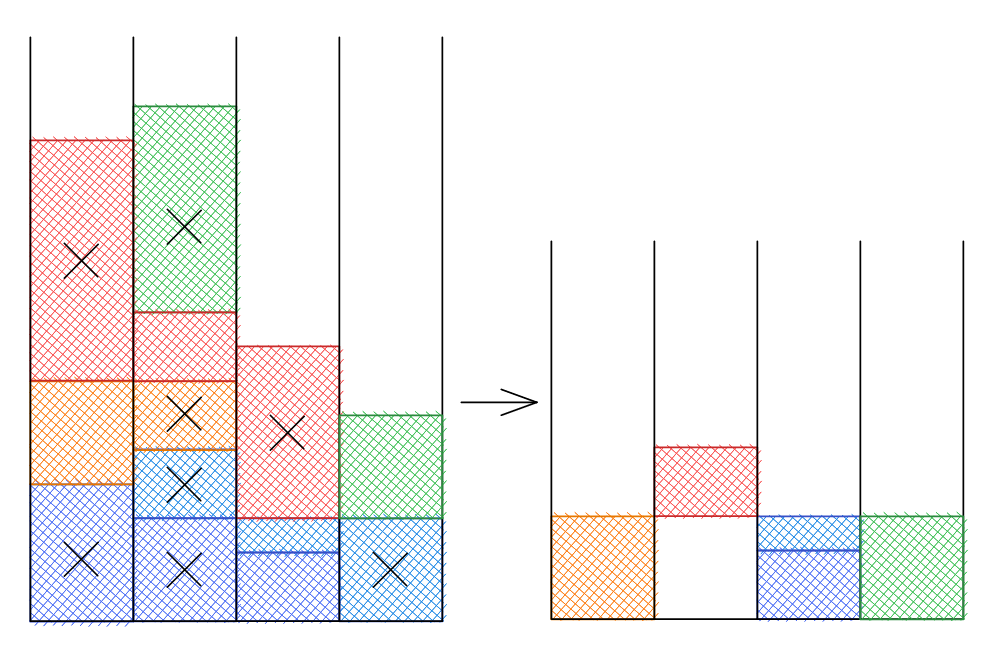
\includegraphics[scale=0.4]{image-rep.png}
    \caption{Representación mediante imagen con eliminación}
    \label{fig:image-rep}
\end{figure}

\subsubsection{Representación con grafos y nodo de cambio de máquina}
Por último, se decidió utilizar una representación basada en grafos, donde cada nodo
representa una operación y las aristas representan las dependencias entre ellas. Esta
representación se basa en la primera representación donde íbamos asignando
operaciones a máquinas, pero en este caso sustituimos esa representación matricial por
una representación mediante grafos. Esta representación no solo soluciona el problema
de la dimensionalidad de la representación, sino que además permite representar de
forma más sencilla las dependencias entre operaciones. Además, se mantiene la idea del
cambio de máquina con un nodo especial que representa el cambio y esta representación
es la que se ha utilizado en las versiones primerizas del modelo final. Esta versión
es muy parecida a la versión final, pero se decidió cambiar el modo en el que se realiza
las predicciones y suprimir la función del cambio de máquina.

\begin{itemize}
    \item \textbf{Espacio de estados:} cada estado se representa por un grafo 
    que representa la configuración actual de una máquina. Cada nodo del grafo puede representar 
    una operación, y las aristas representar las dependencias entre ellas. Se le asignan
    características a los nodos, como el tiempo de procesamiento de la operación o cualquier 
    otra información relevante.
    \item \textbf{Espacio de acciones:} las acciones posibles pueden ser cambiar de máquina 
    o realizar una operación en la máquina actual. Puedes representar las acciones mediante 
    un código que identifique cada operación y la máquina en la que se va a asignar. Por 
    ejemplo, una acción puede estar representada por un código que indique cambiar de máquina o 
    un código que indique realizar una operación específica en la máquina actual.
    \item \textbf{Transición de estado:} la transición de estado ocurren cuando el agente 
    toma una acción y el entorno se actualiza en consecuencia. Cuando se realiza una operación 
    en la máquina actual, el grafo de la máquina se actualiza para reflejar el cambio de estado. 
    Si se decide cambiar de máquina, se utiliza un nodo especial en el grafo para representar 
    la transición a otra máquina.
\end{itemize}
\begin{figure}[ht]
    \centering
    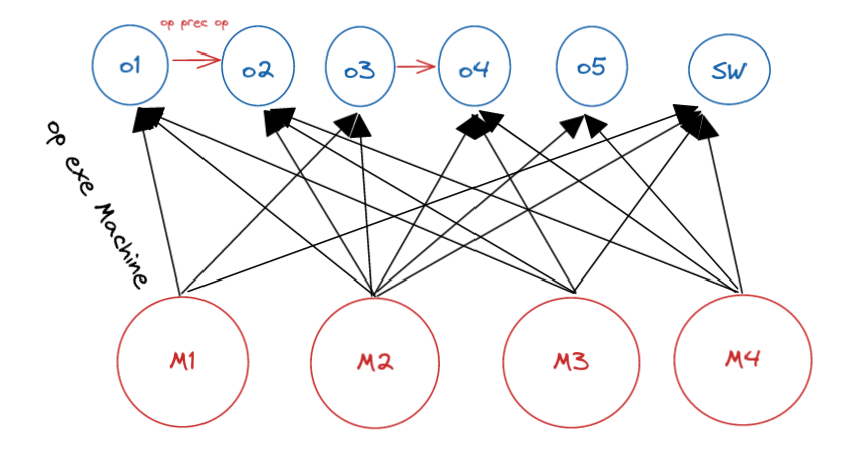
\includegraphics[scale=0.4]{graphv0.png}
    \caption{Representación mediante grafos con nodo de cambio de máquina}
    \label{fig:rep-graph-v0}
\end{figure}


\pagebreak
